\section{Filtros}
\label{sec:filtros}
Filtros são elementos que manipulam amostras de áudio ou vídeos, sendo 
geralmente utilizados para criar efeitos audiovisuais em um pipeline. Eles
sempre possuem pelo menos duas \en{pads}, sendo uma para receber os dados
sobre os quais operam (\en{sink pad}) e outra para escrever os dados 
resultantes do processamento (\en{source pad})\footnote{Alguns filtros possuem 
  mais de uma \en{pad} de entrada e/ou de saída.}. A distribuição oficial do
GStreamer possui vários filtros disponíveis, dentre os quais: \en{volume}
(altera o volume de um fluxo de áudio), \en{videoscale} (altera a resolução de
um fluxo de vídeo), \en{adder} (recebe vários fluxos de áudio e gera um único 
fluxo contendo os sinais de entrada somados), \en{audiokaraoke} (remove a voz
de um fluxo de áudio), etc.

Para demonstrar como podemos adicionar filtros em um \en{pipeline}, vamos 
modificar o programa apresentado na Listagem~\ref{lst:mp3} para fazê-lo 
reproduzir um áudio MP3 com a metade do volume original. O código do reprodutor
de MP3 modificado é apresentado na Listagem~\ref{lst:mp3-volume}.

\lstinputlisting[
style=display,
mathescape=no,
caption={Tocando um arquivo de áudio MP3 com a metade do volume original.},
label={lst:mp3-volume},
]{src/mp3-volume.c}

Note que este programa é bastante semelhante ao programa da
Listagem~\ref{lst:mp3}. A diferença entre ambos está no fato do programa da
Listagem~\ref{lst:mp3-volume} adicionar o filtro \en{volume} ao 
\en{pipeline}. Este filtro é instanciado na linha~21 e está posicionado 
entre o decodificador (\C{mad}) e o \en{sink} (\C{alsasink}). 
Dessa forma, o filtro \en{volume} processa o fluxo de áudio
gerado pelo decodificador e gera um fluxo de áudio modificado para o 
\en{sink}. Na linha~28, a chamada \C{g_object_set} atribui o valor \C{0.5} 
à propriedade ``volume'' do filtro. Essa propriedade controla o nível do 
volume do fluxo de áudio produzido por este filtro, sendo o valor \C{0.0} 
correspondendo ao menor nível (mudo) e \C{1.0} correspondendo ao nível 
máximo  (volume original). Como o valor atribuído é \C{0.5}, o filtro 
processa o fluxo de entrada e gera um fluxo de saída cujo volume é a metade 
do nível original.

Agora vamos criar um programa um pouco mais complexo que permite aos usuários
escolher um entre diversos filtros que adicionam efeitos em um vídeo. 
A Figura~\ref{fig:pipe-filtro} ilustra o \en{pipeline} que vamos construir. 
O programa usa o elemento \C{uridecodebin} para decodificar
um arquivo de vídeo. Se o vídeo possuir fluxo de áudio, este é conectado à
um elemento \C{audioconvert}, que por sua vez é conectado ao elemento
\C{autoaudiosink}. O fluxo de vídeo, por outro lado, é conectado a um filtro
que adiciona algum efeito no vídeo. Note que há um elemento \C{videoconvert}
entre o \C{uridecodebin} e o filtro e outro elemento \C{videoconvert} entre 
o filtro e o \C{autovideosink}. Cada filtro
trabalha com um determinado tipo de \en{caps} em cada uma de suas \en{pads}.
Assim, o fluxo de vídeo gerado pelo \C{uridecodebin} é conectado a um  
elemento \C{videoconvert} que faz as conversões necessárias entre formatos para
garantir que o filtro instanciado receba os dados no formato adequado.
Da mesma forma, o elemento \C{videoconvert} que recebe a saída do filtro e está
conectado ao \C{autovideosink} faz as conversões necessárias para
que este último elemento receba o fluxo também no formato adequado. 
Dessa forma, esse \C{pipeline} nos permite adicionar qualquer filtro de vídeo
sem que haja problema de conexão entre os elementos.

\begin{figure}[H]
  \centering
  \begin{tikzpicture}
    \node (dec) [element] {uridecodebin};
    \coordinate [above=.5\hdim of dec] (A);
    \coordinate [below=.5\hdim of dec] (B);
    \coordinate [right of=dec] (C);

    \node (videoconvert) [element] at (C|-A) {videoconvert};    
    \node (filter) [element, right of=videoconvert] {filtro};
    \node (videoconvert2) [element, right of=filter] {videoconvert};
    \node (autovideosink) [element, right of=videoconvert2] {autovideosink};
    \node (audioconvert) [element] at (C|-B) {audioconvert};
    \node (autoaudiosink) [element, right of=audioconvert] {autoaudiosink};
    \coordinate (X) at ($(dec.east)+(0,.25\hdim)$);
    \coordinate (Y) at ($(dec.east)+(0,-.25\hdim)$);
    \draw [->, arrow] (X) -- node [arrowlabel, above] {V} ++(\odim/3,0)
                          -- ($(videoconvert.west)-(\odim/3,0)$)
                          -- (videoconvert.west);
    \draw [->, arrow] (Y) -- node [arrowlabel, below] {A} ++(\odim/3,0)
                          -- ($(audioconvert.west)-(\odim/3,0)$)
                          -- (audioconvert.west);
    \draw [->, arrow] (videoconvert) -- (filter);
    \draw [->, arrow] (filter) -- (videoconvert2);
    \draw [->, arrow] (videoconvert2) -- (autovideosink);
    \draw [->, arrow] (audioconvert) -- (autoaudiosink);
  \end{tikzpicture}
  \caption{Um \en{pipeline} GStreamer que adiciona diferentes filtros 
    em um vídeo.}
  \label{fig:pipe-filtro}
\end{figure}
\vskip-\baselineskip

A Listagem~\ref{lst:video-filter} apresenta o código de um programa que
implementa o \C{pipeline} acima. O programa usa o argumento \C{argv[1]} para
instanciar um dentre os seguintes filtros:
\C{coloreffects, rippletv, shagadelictv, edgetv} ou \C{revtv}.
A Figura~\ref{fig:video-filter} mostra o resultado da aplicação de cada um
desses filtros.

\lstinputlisting[
style=display,
mathescape=no,
caption={Adicionando diversos efeitos em um vídeo.},
label={lst:video-filter},
]{src/video_filter_v1.c}

\begin{figure*}[h!]
  \centering
  \subfigure[original]{
    
\includegraphics[width=0.4\textwidth]{pics/original}
  }
  \subfigure[coloreffects]{
    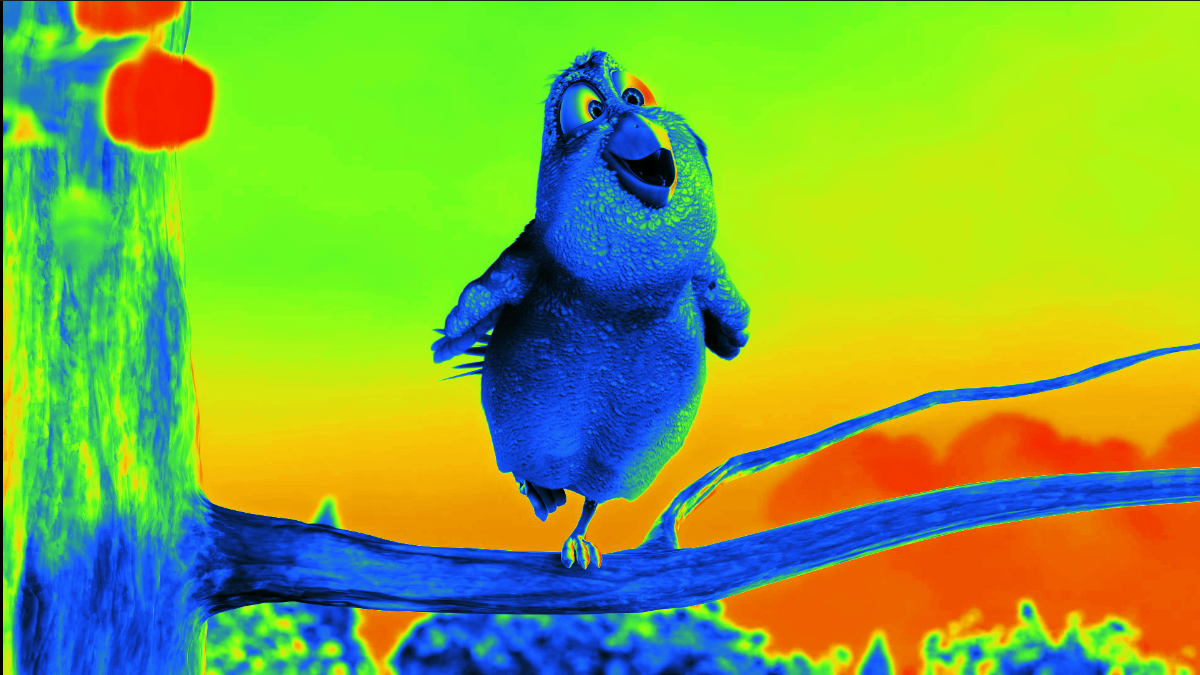
\includegraphics[width=0.4\textwidth]{pics/coloreffects}
  }
  \subfigure[rippletv]{
    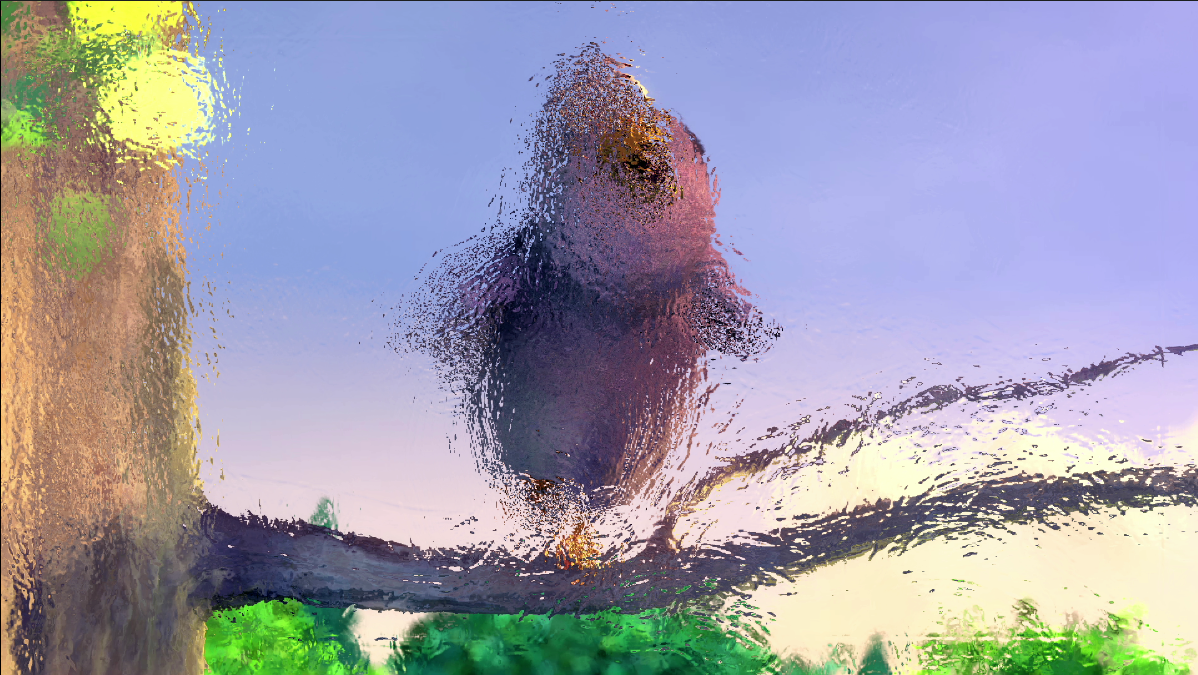
\includegraphics[width=0.4\textwidth]{pics/rippletv}
  }
  \subfigure[shagadelictv]{
    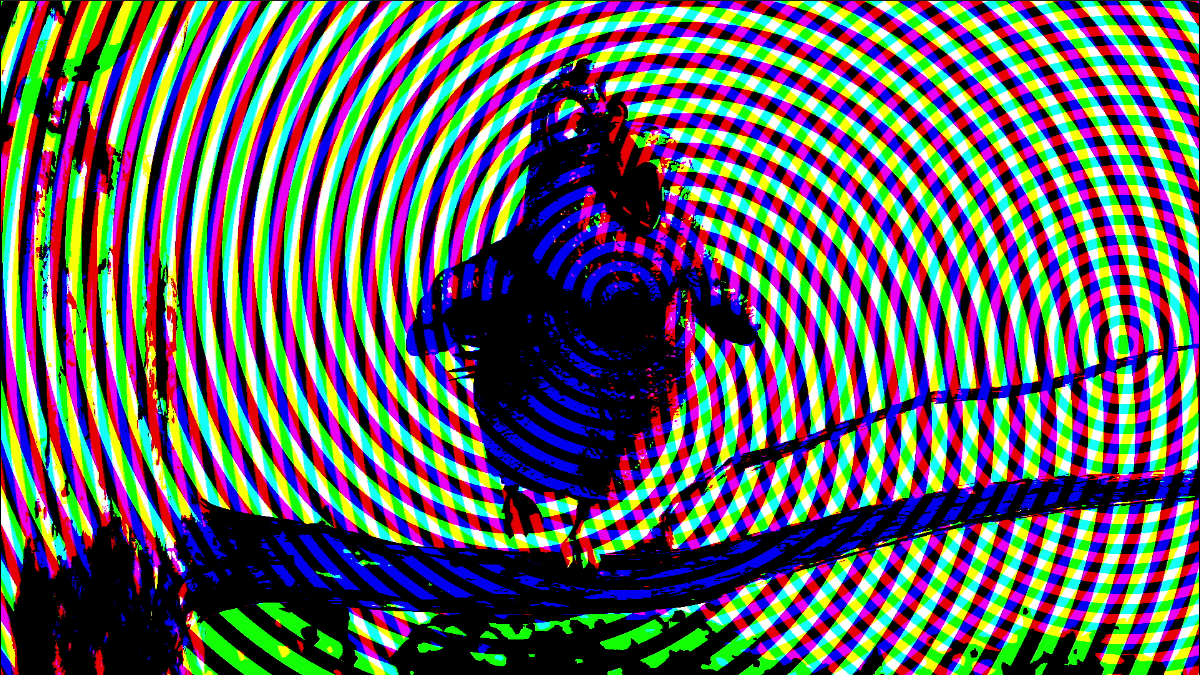
\includegraphics[width=0.4\textwidth]{pics/shagadelictv}
  }
  \subfigure[edgetv]{
    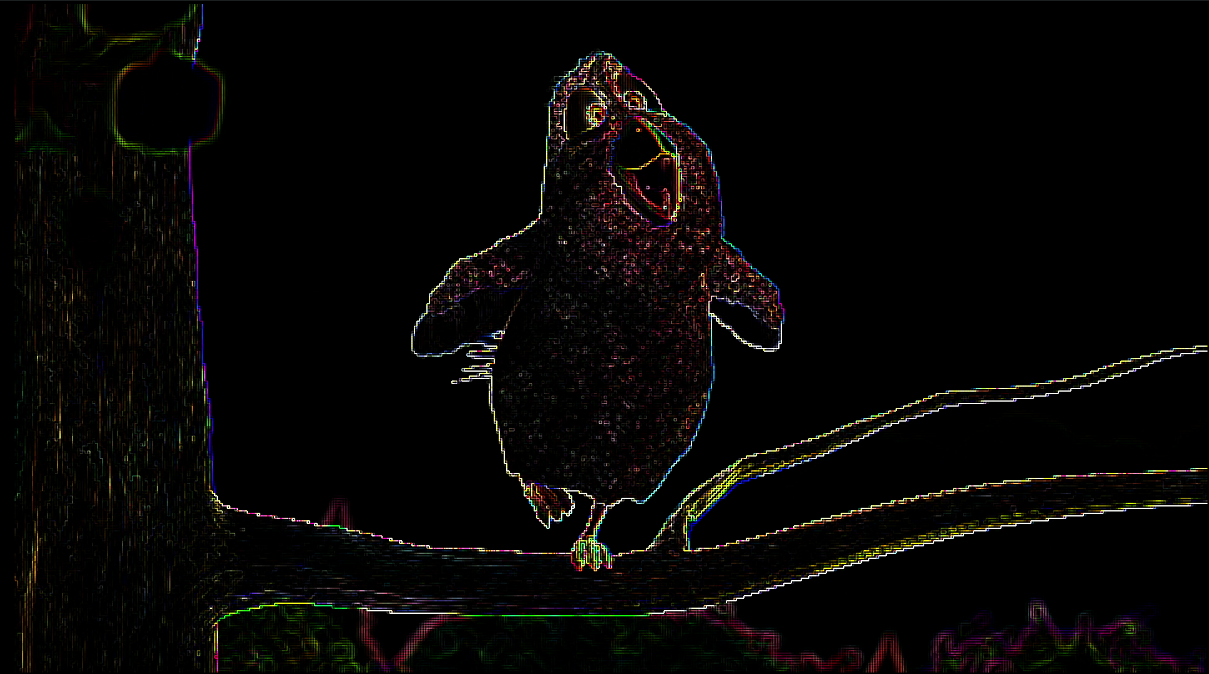
\includegraphics[width=0.4\textwidth]{pics/edgetv}
  }
  \subfigure[edgetv]{
    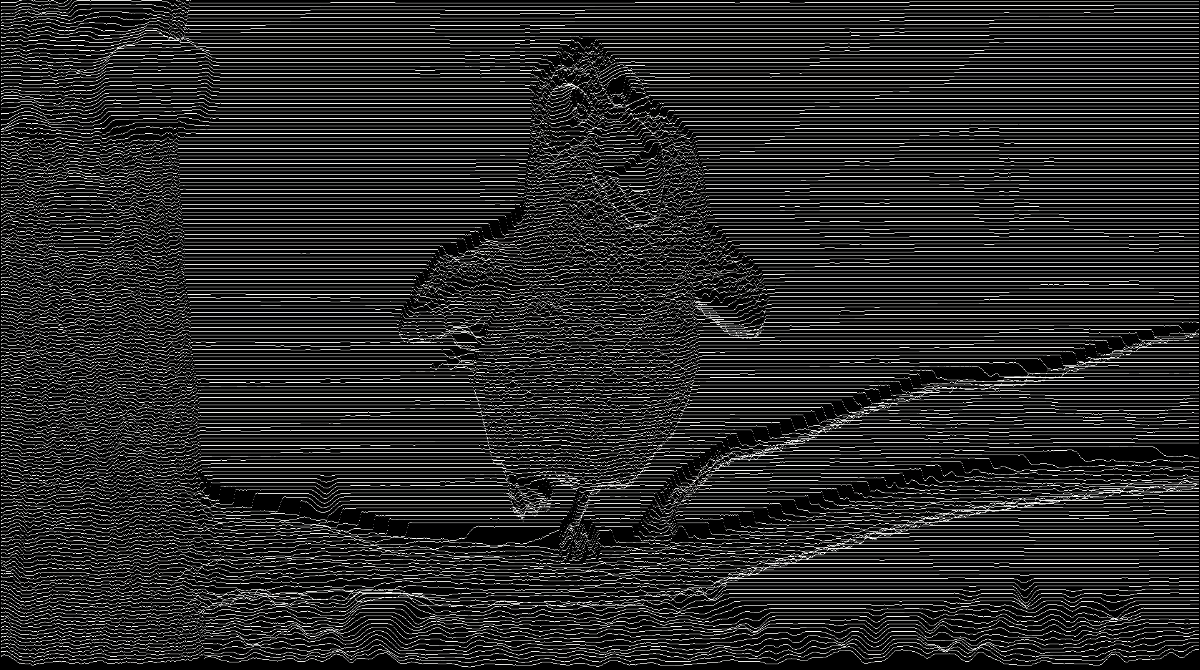
\includegraphics[width=0.4\textwidth]{pics/revtv}
  }
  \caption{Exemplos de filtros que adicionam efeitos à vídeos.}
  \label{fig:video-filter}
\end{figure*}
